\documentclass[12pt]{article} 
\usepackage{geometry} 
\geometry{a4paper} 
\linespread{1.1} % Line spacing


% FIGURES AND FLOATS
\usepackage{graphicx} % Required for including pictures
\usepackage{float} % Allows putting an [H] in \begin{figure} to specify the exact location of the figure
\usepackage{wrapfig} % Allows in-line images such as the example fish picture
\usepackage[font={small,it}]{caption}
\usepackage{subcaption}
\usepackage{epstopdf}
\graphicspath{{images/}}
\usepackage{diagbox}

% MATH
\usepackage{amssymb}
\usepackage{amsmath}
\usepackage{algorithm}
\usepackage[noend]{algpseudocode}

% OTHER
\usepackage[]{mcode}
\usepackage{enumerate}
\usepackage{xcolor}


%character
\usepackage{indentfirst} % 强制要求第一个段落也进行缩进
%段间距
\setlength{\parskip}{1ex plus 0.5ex minus 0.5ex}
%%%%%%%%%%%%%%%%%%%%%%%%%%%%%%%%%%%%%%%%%%%%%%%%%%%%%%%%%%%%
\usepackage{listings} 

%段首缩进
\setlength{\parindent}{2em} 

\definecolor{DeepPink}{RGB}{255, 20, 147}
\definecolor{LightSlateBlue}{RGB}{132, 112, 255}
\definecolor{ForestGreen}{RGB}{34, 139, 34}

\lstset{
  language=Matlab,  %代码语言使用的是matlab
  frame=shadowbox, %把代码用带有阴影的框圈起来
  rulesepcolor=\color{red!20!green!20!blue!20},%代码块边框为淡青色
  keywordstyle=\color{blue!90}\bfseries, %代码关键字的颜色为蓝色,粗体
  commentstyle=\color{ForestGreen}\textit,    % 设置代码注释的颜色
  showstringspaces=false,%不显示代码字符串中间的空格标记
  numbers=left, % 显示行号
  numberstyle=\tiny,    % 行号字体
  stringstyle=\ttfamily, % 代码字符串的特殊格式
  basicstyle={\small\ttfamily},
  breaklines=true, %对过长的代码自动换行
  extendedchars=false,  %解决代码跨页时,章节标题,页眉等汉字不显示的问题
  texcl=true,
  % basicstyle=\fontfamily{Microsoft YaHei}\selectfont\footnotesize, % 设置字体族为微软雅黑,字号为footnotesize
}

\lstset{breaklines}%自动将长的代码行换行排版

\lstset{extendedchars=false}%解决代码跨页时,章节标题,页眉等汉字不显示的问题
%%%%%%%%%%%%%%%%%%%%%%%%%%%%%%%%%%%%%%%%%%%%%%%%%%%%%%%%%%%%
\title{\LARGE Solution to analysis in Home Assignment 4 \\  \vspace{1cm}\Large }
\author{Yongzhao Chen(yongzhao@chalmers.se)}
\date{\vspace{8cm}\today}
\begin{document}
\maketitle
\thispagestyle{empty}
\newpage
%%%%%%%%%%%%%%%%%%%%%%%%%%%%%%%%%%%%%%%%%%%%%%%%%%%%%%%%%%%%
\section{Part 2}
\subsection{How to design LQI controller}

A stationary LQR can be used to find the feedback control gain K, which minimizes thefollowing quadratic cost, with respect to a control input u(t):

\begin{equation}
    \begin{aligned}
        J=\dfrac{1}{2}\int_0^\infty\left(x(t)^TQ_xx(t)+u(t)^TQ_uu(t)\right)dt
    \end{aligned}
\end{equation}

where $ Q_x $ and $ Q_u $ are weighting matrices, telling the controller about  the priorities of tunning states and control signals.

The original LQR method can be extended to achieve reference tracking. To do this, the system needs to be augmented with integral states $z_i$, which allow the computation of the cumulative tracking error $ \int (y-r)dt $ :
\begin{equation}
    \begin{aligned}
        \begin{bmatrix}
             \dot{x}(t)\\\dot{z}(t)\end{bmatrix}=\underbrace{\begin{bmatrix}A_\delta&0\\C_I&0\end{bmatrix}}_{A_{aug}}\begin{bmatrix}x(t)\\z(t)\end{bmatrix}+\underbrace{\begin{bmatrix}B_\delta\\0\end{bmatrix}}_{B_{aug}}u(t)+\begin{bmatrix}K_r\\-I\end{bmatrix}r(t)
    \end{aligned}
\end{equation}

\begin{equation}
    \begin{aligned}
        u(t)=-K\begin{bmatrix}x(t)\\z(t)\end{bmatrix}=-[K_PK_I]\begin{bmatrix}x(t)\\z(t)\end{bmatrix}
    \end{aligned}
\end{equation}

where $C_I$ selects the system states needed to compute the new integral states, and $ K $ can be calculated by Matlab function \texttt{lqr}.

\subsection{Application and verify}

For the assignment 1 part 2, the system does not have other input singals expect a singal reference signal $ \mathbf{r} $.

The augmented system is :
\begin{equation}
    \begin{aligned}
        &\begin{bmatrix}\dot{x}\\\dot{x}_i\end{bmatrix}=\begin{bmatrix}A&0\\-C&0\end{bmatrix}\begin{bmatrix}x\\x_i\end{bmatrix}+\begin{bmatrix}B\\0\end{bmatrix}u+\begin{bmatrix}0\\0\\0\\0\\1\end{bmatrix}r\\
        &\mathbf{A_{aug}} = \begin{bmatrix}A&0\\-C&0\end{bmatrix} \\
        &\mathbf{B_{aug}} = \begin{bmatrix}0\\0\\0\\0\\1\end{bmatrix}
    \end{aligned}
\end{equation}

where $ \mathbf{C} $ is selected as $ \mathbf{C(1,:)} $, since $\mathbf{y = Cx }$ and $ y_1=\alpha $.

Select $Q,  R$ after tunning:

\begin{lstlisting}
    Q = diag([0 100 0 0 0 1]);
    R = diag([1 1 1]);       
\end{lstlisting}

And use the build- in function to get the $ K $ matrix:

\begin{lstlisting}
    [K,~ ,~] = lqr(A_aug, B_aug, Q, R)
\end{lstlisting}

Now rebuild the new closed loop feedback system as :

\begin{lstlisting}
    Ae = [A_lqr-B_lqr*K]; % 6x6
    Be = [0 0 0 0 0 1]'; % 6x1
    Ce = [C zeros(3, 1)]; % 3x6
    De = 0; % 1x1
    sys_e = ss(Ae, Be, Ce, De);
\end{lstlisting}

The respond of a step signal shows below:

\begin{figure}[H]
 \centering
 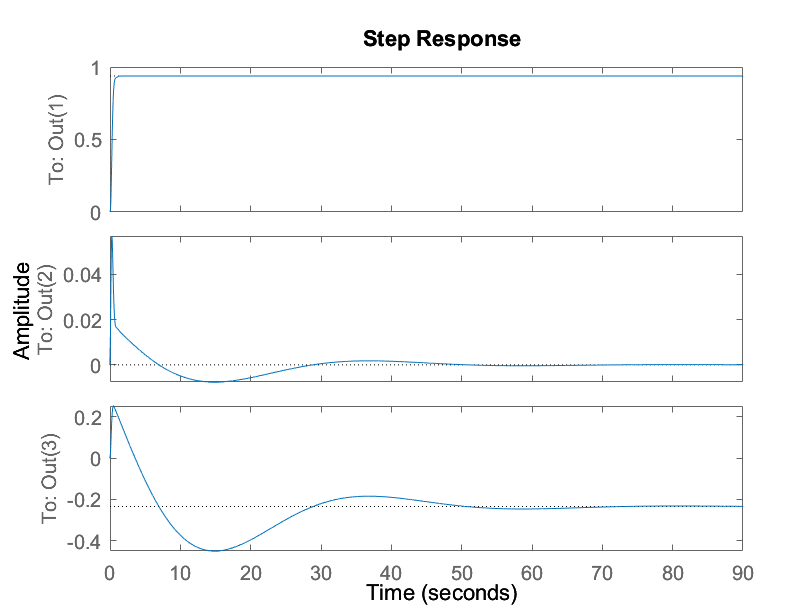
\includegraphics[width=0.8\textwidth]{images/step.png}
 \caption{Step respond}
 \label{step}
\end{figure}

From the picture \ref{step}, it is clear we achieved a reference tracking for the state $ \alpha $.

  

\begin{equation}
    \begin{aligned}
        \begin{bmatrix}
            y\Delta\\z_e\\z_p\\z_u\\v_r\\v_\tilde{y}
            \end{bmatrix}
            =
            \begin{bmatrix}
                0           & 0           & 0            & 0   & G_a \\
                -W_eG_nW_m  & -W_eG_nW_d  & W_eW_{r\alpha}  & 0   & -W_eG_nG_a\\
                W_pG_nW_m   & W_pG_nW_d   & 0               & 0   & W_pG_nG_a\\
                W_uW_m      & W_uW_d      & 0               & 0   & W_uW_a\\
                0           & 0           & I               & 0   & 0\\
                G_nW_m      & G_nW_d      & 0               & W_n & G_nG_a\\
            \end{bmatrix}
            =
            \begin{bmatrix}
                u\Delta\\d\\r\\n\\u
            \end{bmatrix}
    \end{aligned}
\end{equation}
\input{Q3.tex}
\input{Q4.tex}
%%%%%%%%%%%%%%%%%%%%%%%%%%%%%%%%%%%%%%%%%%%%%%%%%%%%%%%%%%%%%
\end{document}
